\documentclass{beamer}

\usepackage[ngerman]{babel}
\usepackage[utf8]{inputenc}
\usepackage[T1]{fontenc}
\usepackage{lmodern}

\usepackage[german,linesnumbered,algoruled,longend,vlined]{algorithm2e}
\DontPrintSemicolon
\SetArgSty{}
\SetKw{KwOr}{or}
\SetKw{KwAnd}{and}
\SetKw{KwNot}{not}
\setlength{\algomargin}{3ex}

\usepackage[fixlanguage]{babelbib}
\setbibliographyfont{title}{}
\setbibliographyfont{jtitle}{}
\setbibliographyfont{btitle}{\emph}
\setbibliographyfont{stitle}{\emph}
\setbibliographyfont{journal}{\emph}

\usepackage{amsmath}
\usepackage{amsfonts}
\usepackage{amssymb}
\usepackage{amsthm}

\usepackage{graphicx}
\usepackage{enumerate}
\usepackage{textcomp}
\usepackage{epstopdf}

\graphicspath{{graphics/}}

% Eigene Commands:
\newcommand{\Epsilon}{\mathcal{E}}
\newcommand{\N}{\mathbb{N}}

\hyphenation{Teil-as-pekt Teil-as-pek-te}

\begin{document}



\subject{Algorithmen für geographische Informationssysteme}
\title{Projekt Viewshed Analysis}
\author{Christina Hempfling, Jona Kalkus, Moritz Beck, Bernhard Häussner}
\date{Projekt-Präsentation am 15. Juni 2015}
\institute{Julius-Maximilians-Universität Würzburg\\
Institut für Informatik\\
Lehrstuhl für Informatik I\\
Effiziente Algorithmen und wissensbasierte Systeme\\[\baselineskip]
Betreuer:\\ 
Prof.\ Dr.\ Alexander Wolff\\
Dr.\ Thomas van Dijk\\
Benedikt Budig, M.Sc.}
\maketitle


\section{Einleitung}

\begin{frame}
  \frametitle{Ein Beispiel für Viewshed Analysis}
  \begin{figure}[h]
    \centering
    \fbox{\includegraphics<1>[height=5cm]{berg_viewpoint}\includegraphics<2>[height=5cm]{berg_viewshed}}
    \caption{Ein Digitales Höhenmodell (DEM) \only<2>{mit Viewshed}}
    \label{fig:example}
  \end{figure}
\end{frame}

\begin{frame}
  \frametitle{Was ist Viewshed Analysis?}
  \begin{itemize}[<+->]
    \item Eingabe:
    \begin{itemize}
      \item Digitales Höhenmodell (DEM)
      \item Standpunkt im DEM
      \item Höhe im DEM
    \end{itemize}
    \item Ausgabe: Sichtbarer Bereich vom Standpunkt aus
    \item Anwendungen: 
    \begin{itemize}
      \item Aufstellen von Sendemasten
      \item Finden versteckter Routen
      \item Finden landschaftlich attraktiver Routen
    \end{itemize}
  \end{itemize}
\end{frame}

\section{Algorithmen}

\begin{frame}
  \frametitle{Der naive Algorithmus}
  \begin{itemize}
    \item Für jeden Punkt des DEM:
    \begin{itemize}
      \item Finde alle Punkte zwischen diesem und dem Standpunkt
      \item Prüfe für diese Punkte, ob sie größere Steigung haben
      \item Hat keiner größere Steigung, ist der Punkt sichtbar
    \end{itemize}
    \item<2-> Laufzeit $O(n^3)$ ($n :=$ Maximum aus Breite u. Höhe des DEM)
    \item<3-> Laufzeit unseres Java-Programms ca. 10 s auf 500x1000 Pixeln
    \item<4-> Lässt sich sehr leicht implementieren und parallelisieren
  \end{itemize}
\end{frame}


\begin{frame}
  \frametitle{Verbesserung: Sweepline (van Krefeld~\cite{van1996variations})}
  \begin{itemize}
    \item Radiale Sweepline (wie auf einem Radarschirm)
    \item Events bei Beginn, Mitte und Ende eines Pixels, nach Winkel sortiert
    \item Baumstruktur speichert Punkte aktuell auf Sweepline, erlaubt schnelles Sichtbarkeits-Prüfen
    \item<2-> Laufzeit $O(n^2 \log{n})$ ($n$ Breite des DEM)
  \end{itemize}
\end{frame}


\begin{frame}
  \frametitle{Verbesserungsidee: Auflösungsvariation, Quad Trees}
  \begin{figure}[h]
    \centering
    \fbox{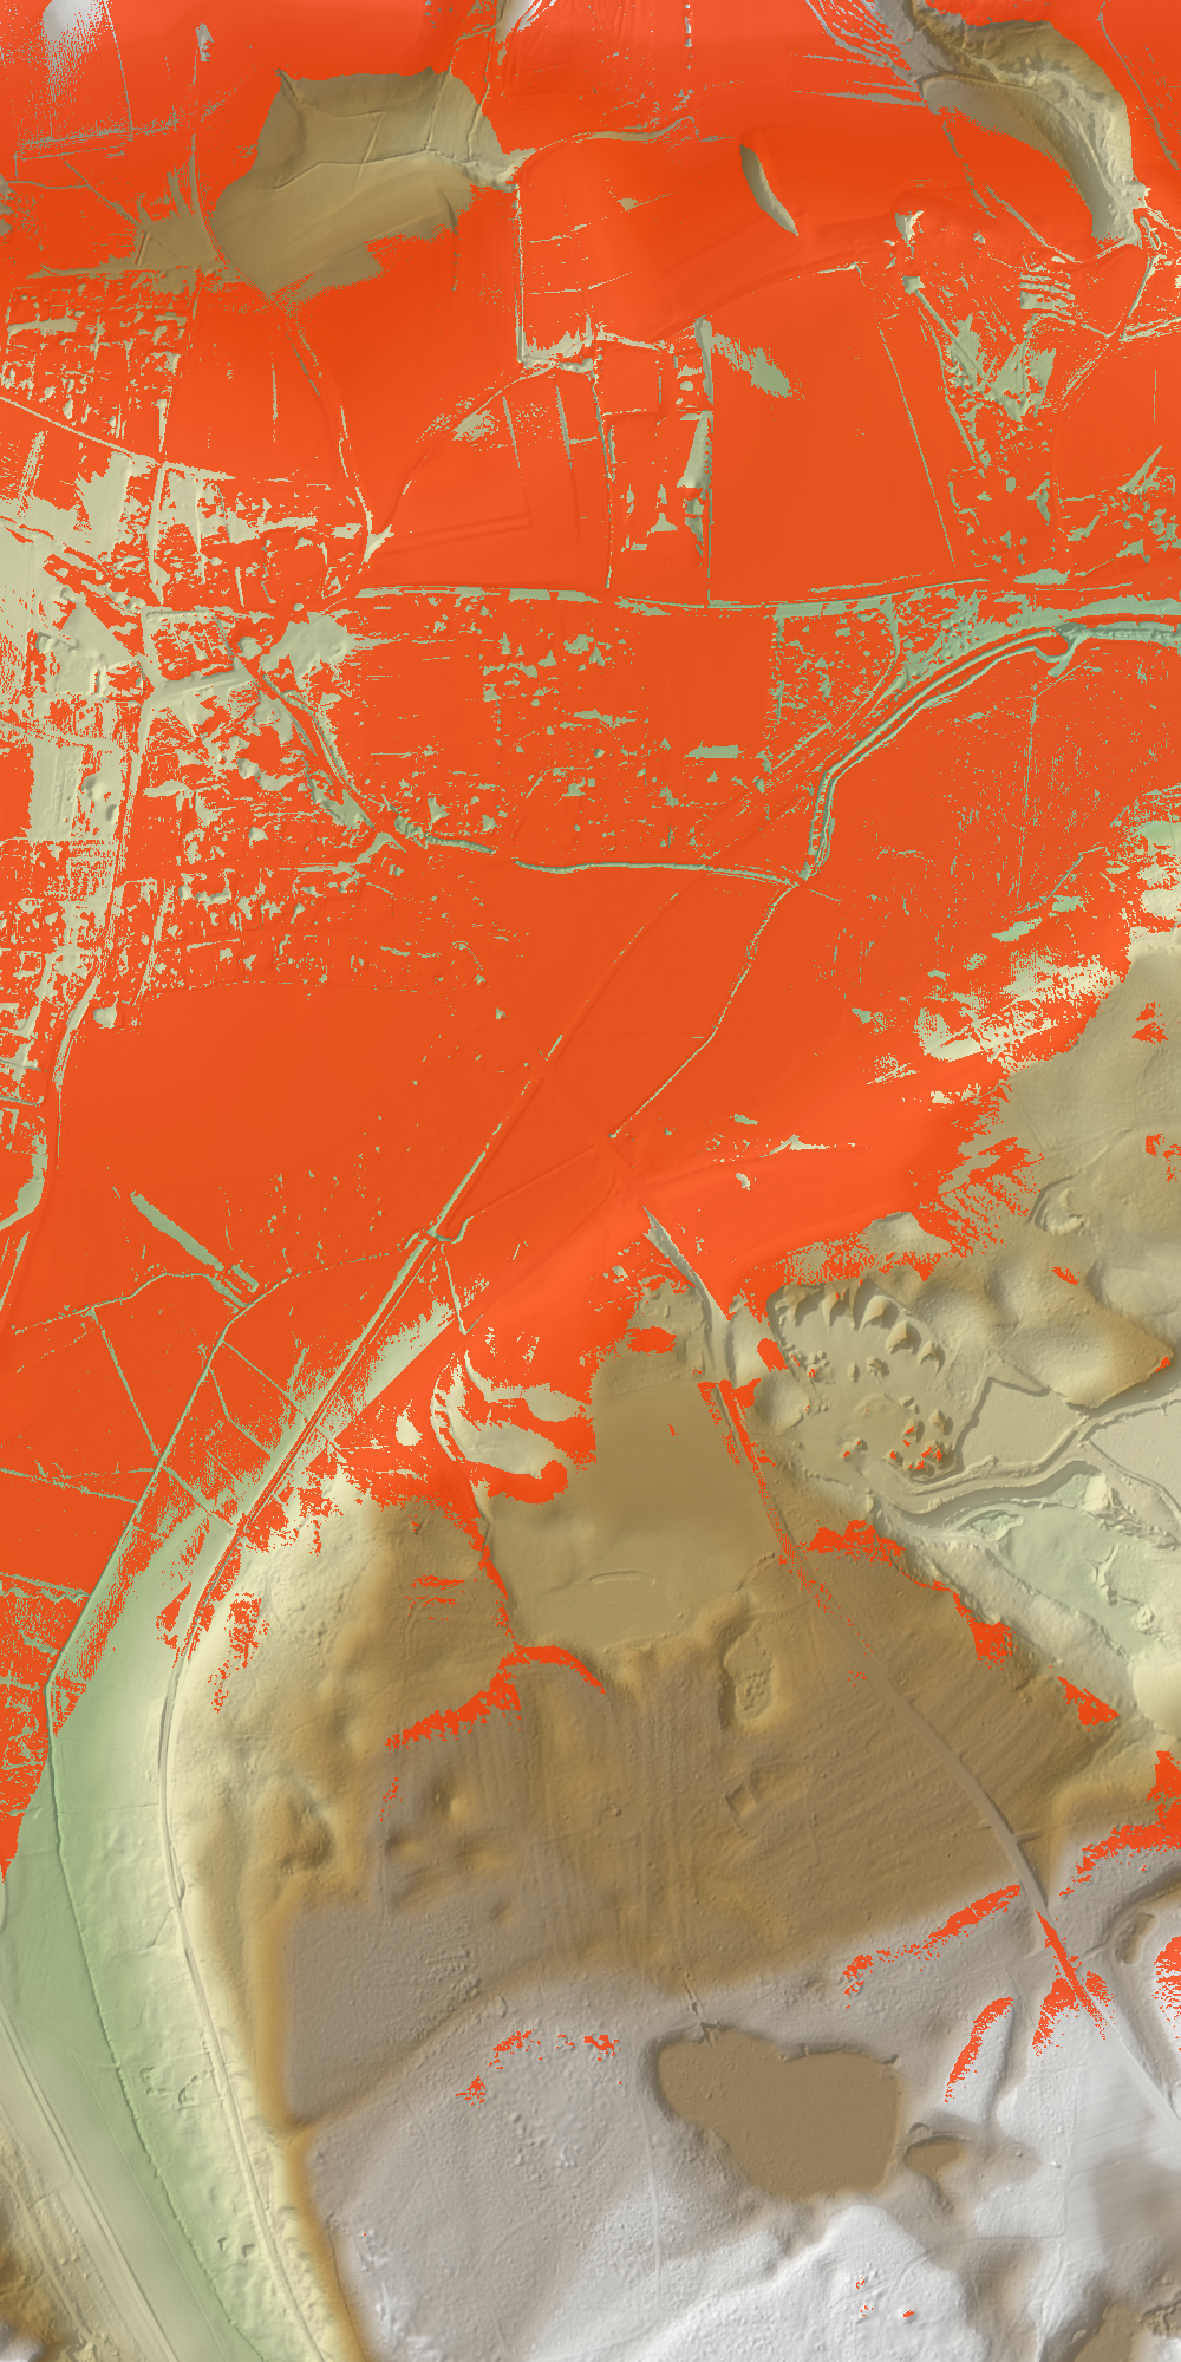
\includegraphics[height=5cm]{dgm_1}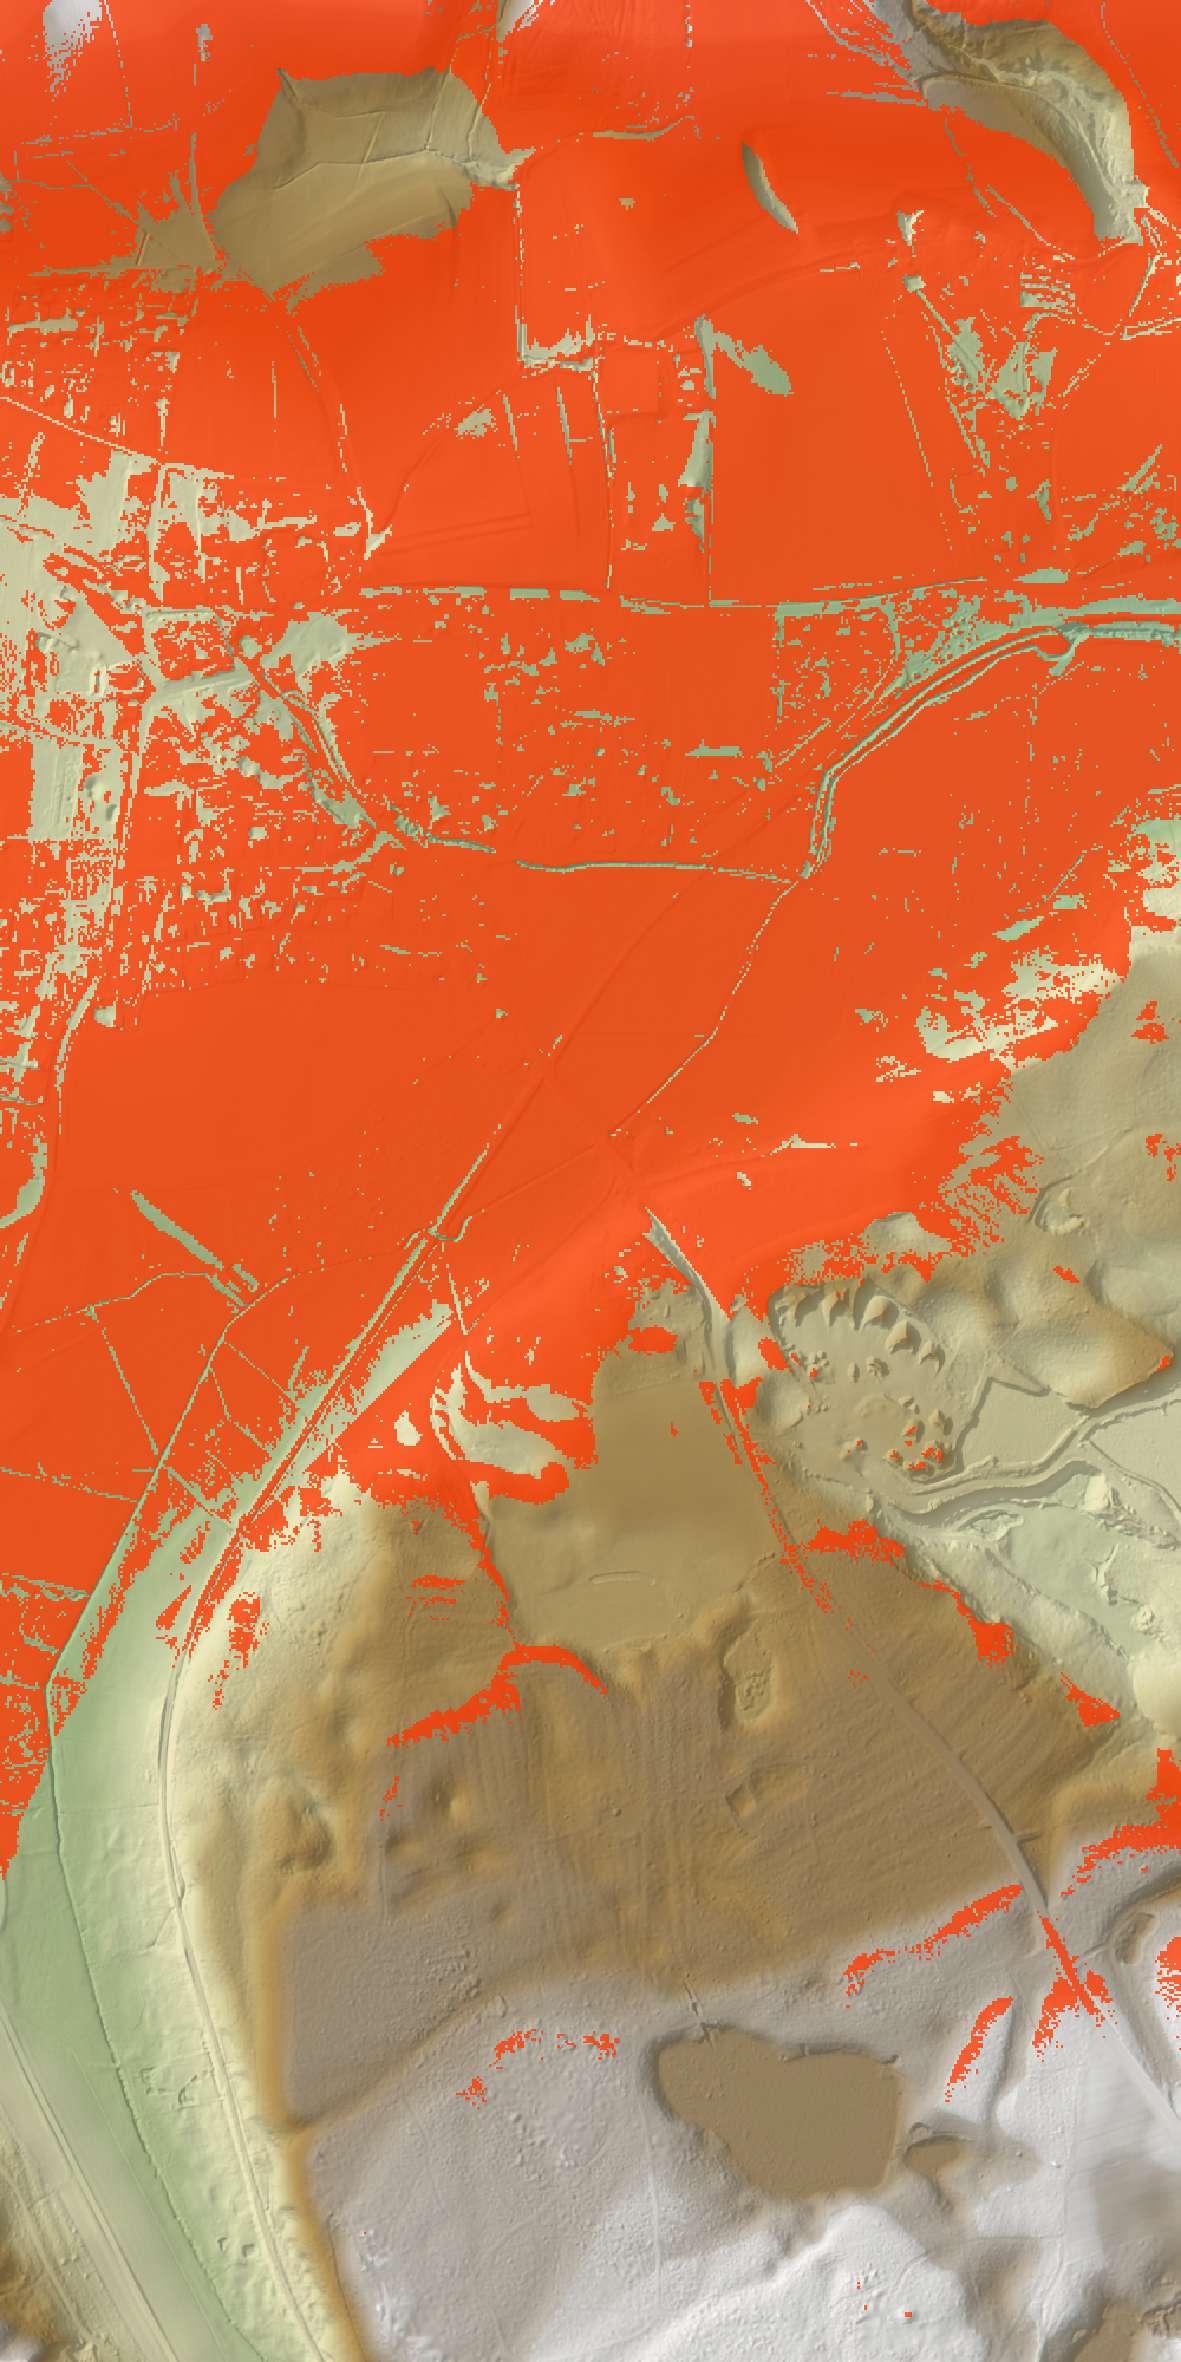
\includegraphics[height=5cm]{dgm_2}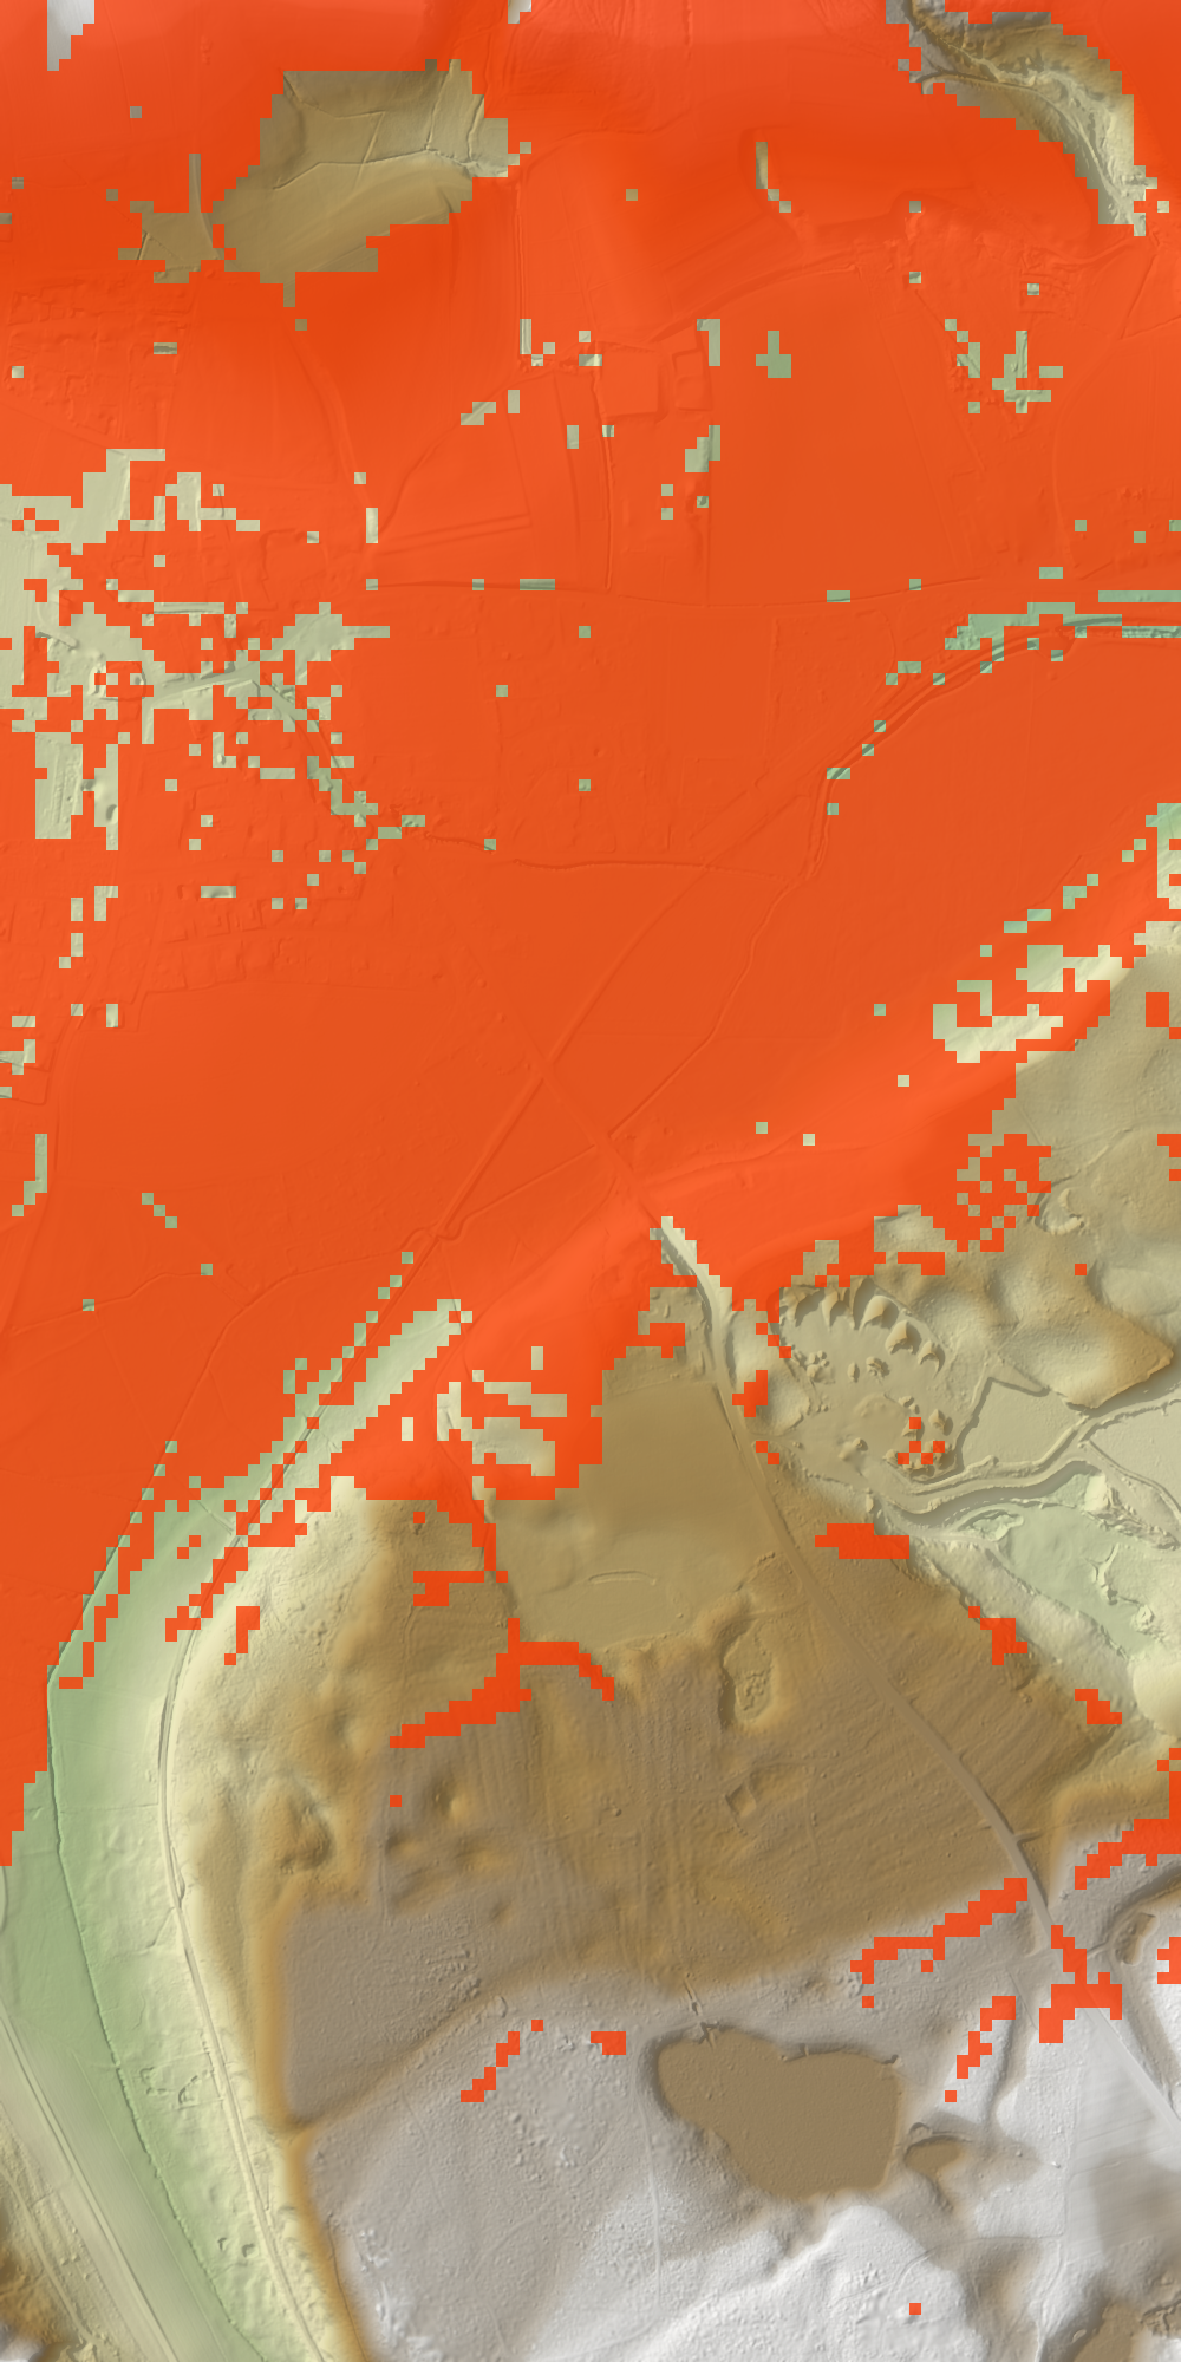
\includegraphics[height=5cm]{dgm_10}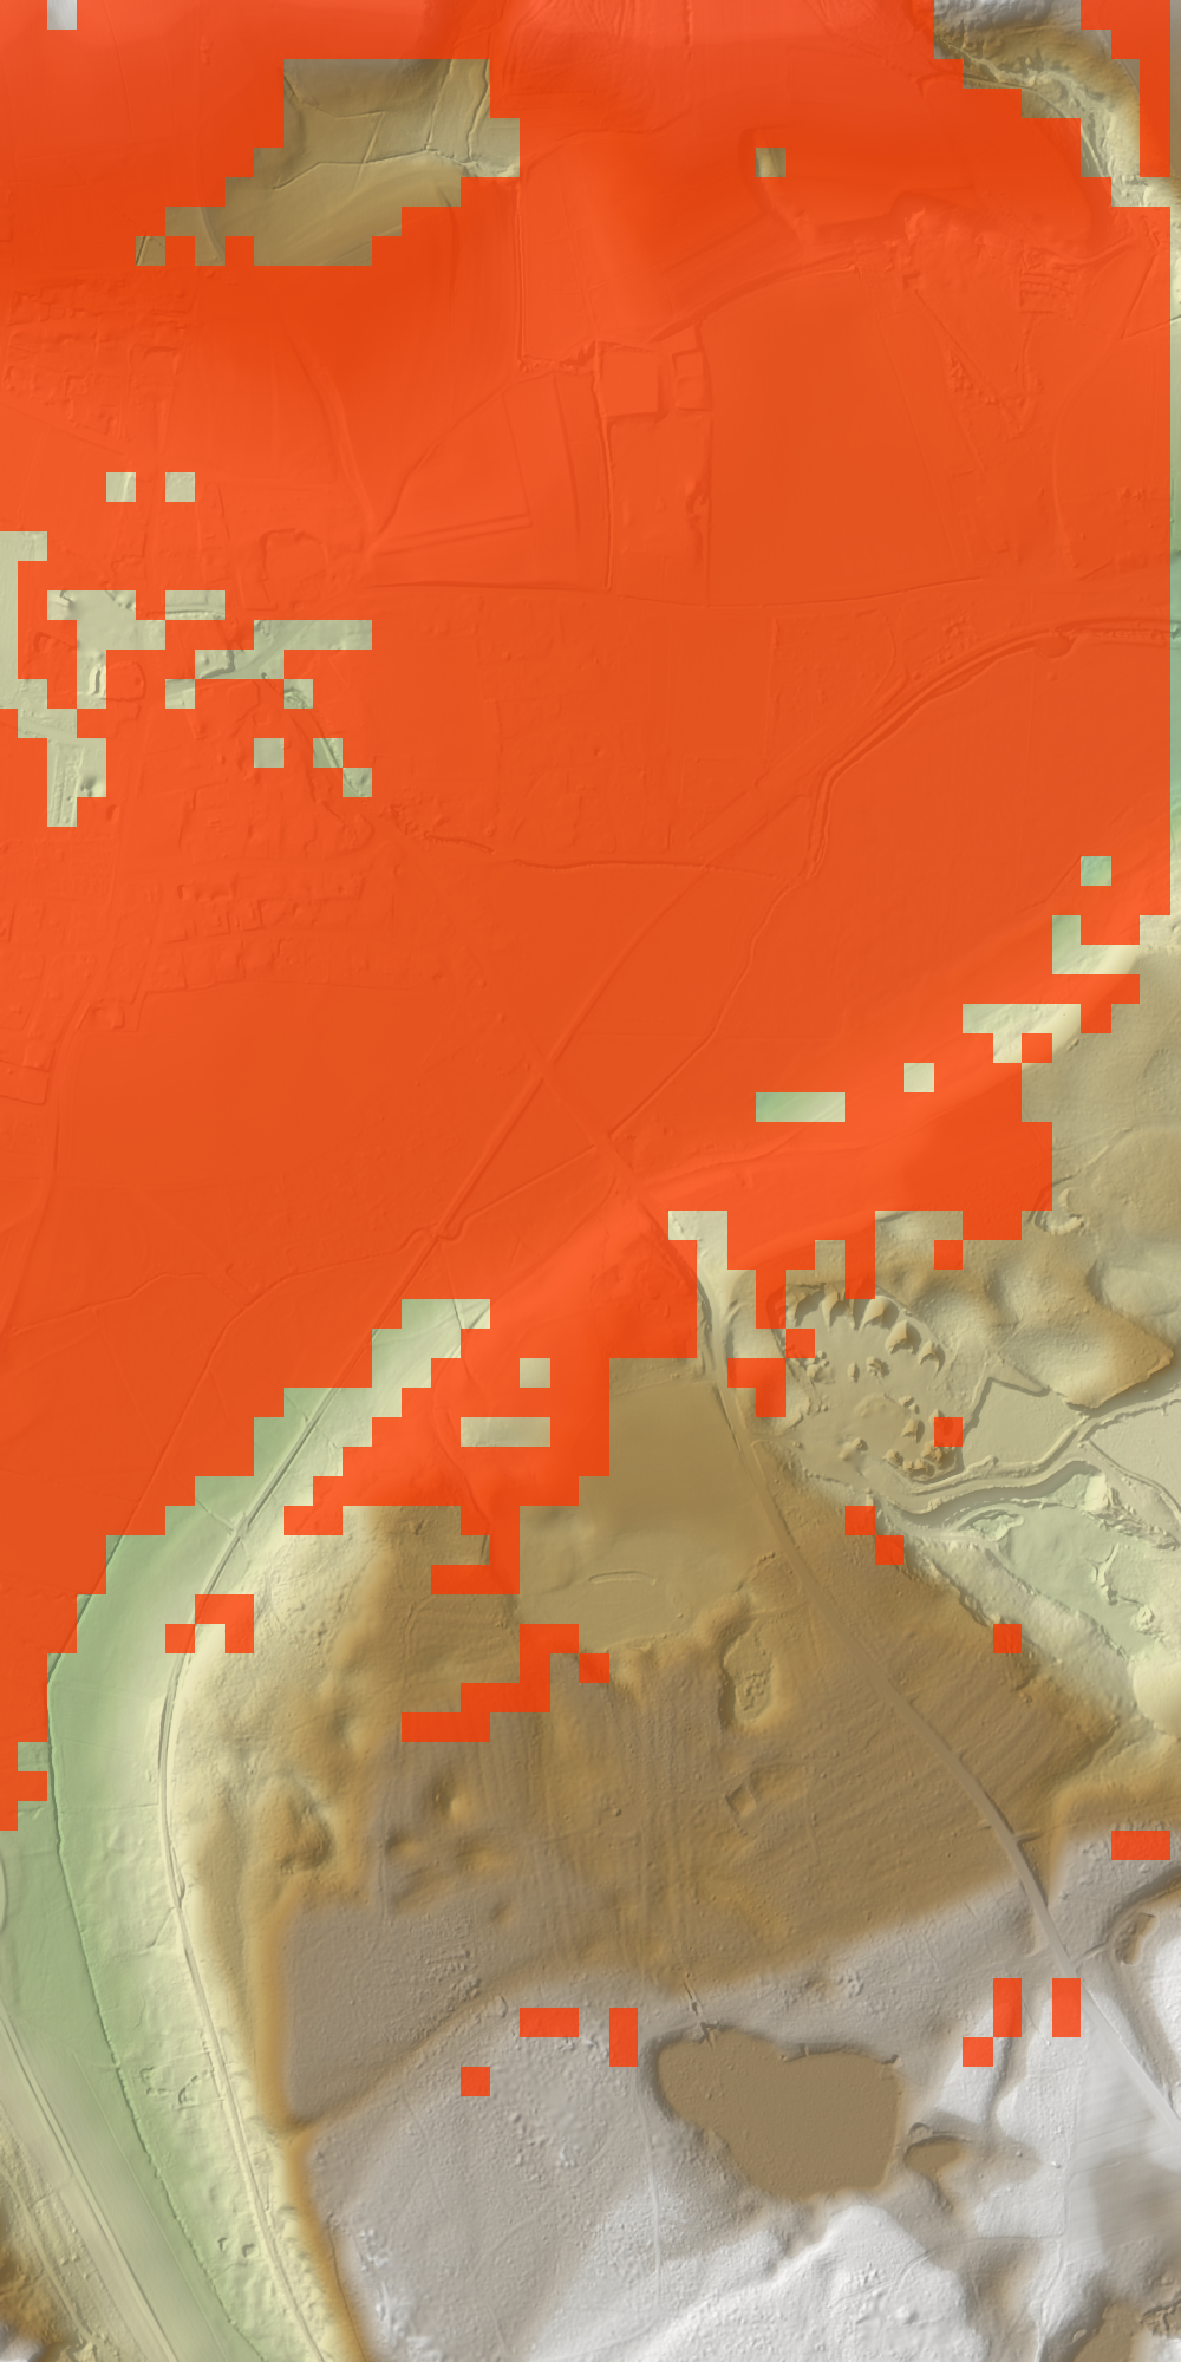
\includegraphics[height=5cm]{dgm_25}}
    \caption{1, 2, 10 und 25 Meter Auflösung. \newline Laufzeit: 151, 17, 0.16, 0.03 Sekunden}
    \label{fig:example}
  \end{figure}
\end{frame}

\section{Probleme}

\begin{frame}
  \frametitle{Probleme: Interpolation des DEM~\cite{fisher1993algorithm}}
  \begin{itemize}[<+->]
    \item DEM als Rasterdaten lässt undefinierte Zwischenräume
    \item Interpolation naher Pixel kann große Auswirkungen auf ferne Pixel haben
    \item Pixel könnten z.B. mit einer Wahrscheinlichkeit gesehen werden
  \end{itemize}
\end{frame}

\begin{frame}
  \frametitle{Probleme: Artefakte an Winkelhalbierenden}
  \begin{itemize}[<+->]
    \item 
    \item 
    \item 
    \item 
  \end{itemize}
\end{frame}

\begin{frame}%[shrink=30]
  \frametitle{Literatur}
  \bibliographystyle{mybabalpha-fl}
  \small\bibliography{mybib}
\end{frame}




\end{document}